\section{Durchführung}
\label{sec:Durchführung}

\subsection{Versuchsaufbau}

In der Versuchsreihe wird der in \autoref{Abb:Versuchsaufbau} gezeigte Aufbau verwendet.

\begin{figure}
    \centering
    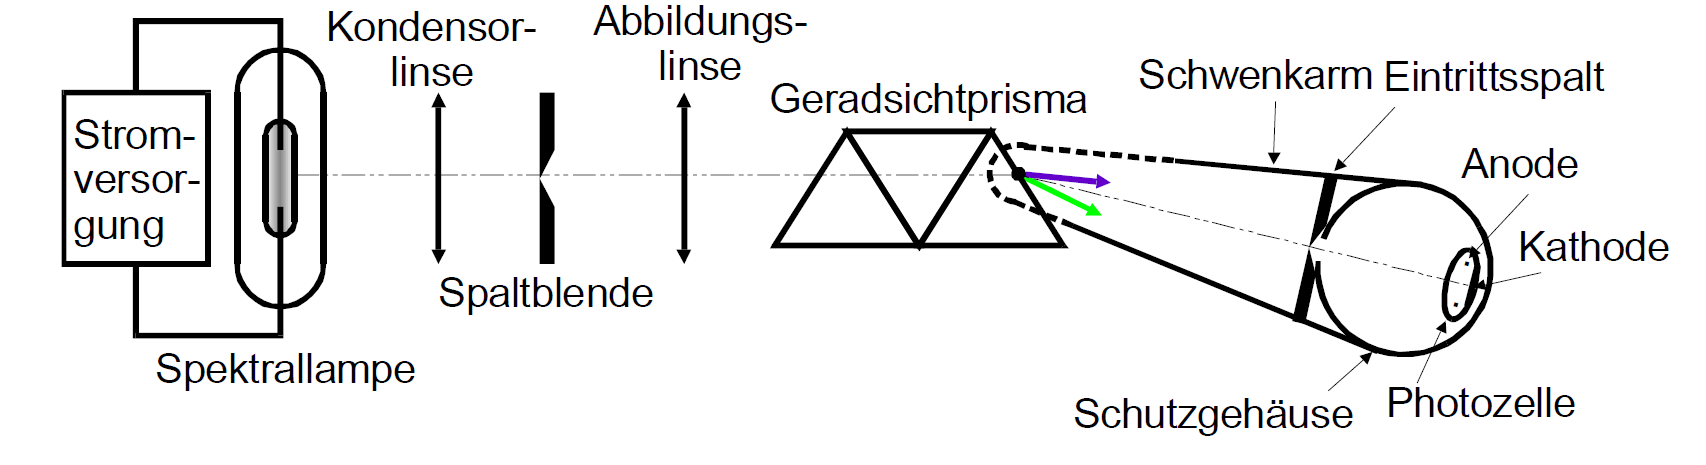
\includegraphics[width=15cm]{Bilder/Versuchsaufbau.png}
    \caption{Verwendeter Versuchsaufbau in beiden Teilversuchen (optischer Teil).\cite{sample}}
    \label{Abb:Versuchsaufbau}
\end{figure}

Die Quecksilber-Spektrallampe wird mit Strom versorgt und erzeugt Licht mit einem für Quecksilber
spezifischen Spektrum. Diese spezifischen Frequenzen sind in \autoref{Tab:HG_Spektrum} abzulesen.

\begin{figure}
    \centering
    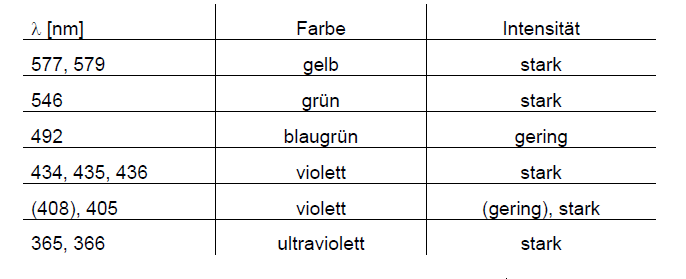
\includegraphics[width=15cm]{Bilder/Hg_Spektrum.png}
    \caption{Die dominantesten Linien im Hg-Spektrum.\cite{sample}}
    \label{Tab:HG_Spektrum}
\end{figure}

Das erzeugte Licht wird in der Kondensorlinse gebündelt und fällt auf die Spaltblende. 
Die danach geschaltete Abbildungslinse entwirft nun ein Bild der Spaltblendenöffnung
auf den Eintrittsspalt der Photokathode.\\
Danach durchläuft das Licht ein Geradsichtprisma, wodurch die einzelnen enthaltenen Frequenzen
optisch getrennt werden. Somit sind auf der Mattscheibe vor der Photokathode nun die einzelnen
Spektallinien zu beobachten.\\
Die Kathode kann nun mit einem Schwenkarm so geschwenkt werden, sodass jeweils nur eine 
Spektrallinie auf den Eintrittsspalt fällt.\\
Um Gegenfelder und Beschleunigungssfelder zu erzeugen und den Strom zu messen, wird außerdem
der in \autoref{Abb:StromZeug} verwendete Versuchsaufbau verwendet.

\begin{figure}
    \centering
    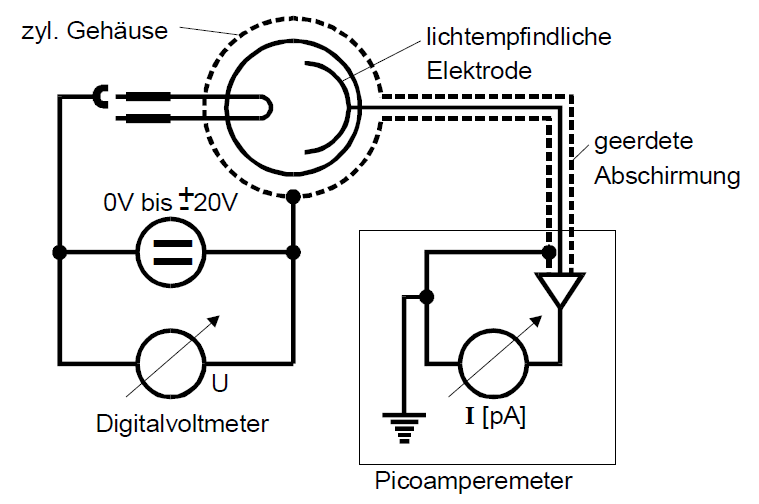
\includegraphics[width=15cm]{Bilder/StromZeug.png}
    \caption{Verwendeter Versuchsaufbau in beiden Teilversuchen (elektrisches Schaltbild).\cite{sample}}
    \label{Abb:StromZeug}
\end{figure}

An die Kathoden-Anoden-Strecke wird eine variable Spannung angeschlossen, wo entweder eine Bremsspannung
oder eine Beschleunigungsspannung verwendet werden kann. Mit einem Picoamperemeter kann nun der Strom 
gemessen werden, welcher von der Kathode zur Anode fließt.

\subsection{Zusammenhang zwischen der Wellenlänge und der Maximalenergie der emittierten Elektronen}

Für die Messungen mit einer angelegten Gegenspannung werden jeweils die rote, gelbe, grüne und zwei
violette Spektrallinien verwendet.\\
Es wird die Abhängigkeit des fließenden Stroms zur angelegten Bremsspannung gemessen, bis kein Strom 
mehr fließt. Es werden ausreichend kleine Schritte verwendet.

\subsection{Abhängigkeit des Elektronenstroms von der angelegten Spannung}

Für das gelbe Licht ($\lambda = $ 578 nm) wird der Photostrom in Abhängigkeit einer angelegten Spannung gemessen. Hier werden sowohl
Beschleunigungsspannung als auch Bremsspannung verwendet im Bereich von $- 20 \, \mathrm{V} \leq U \leq + 20 \, \mathrm{V}$.
Es muss darauf geachtet werden, die Lichtintensität konstant zu halten.

\newpage